
%=============== 2 sous-figures alignées horizontalement =================

\ifx \twoFig \undefined
\def \twoFig [#1]#2#3#4#5#6#7#8#9%
{
\begin{figure}[#1]
\begin{center}
  \subfigure[#2]{\includegraphics[width=#4, page=#6]{figs/figures}}\hspace{1cm}
  \subfigure[#3]{\includegraphics[width=#5, page=#7]{figs/figures}}\hspace{1cm}
  \caption{#8}  % legende \\
  \label{#9} % pour citer le numéro de figure
\end{center}
\end{figure}
}
\fi

%=============== 3 sous-figures alignées horizontalement =================

\ifx \threeFig \undefined
\def \threeFig [#1]#2#3#4#5#6#7#8#9%
{
\begin{figure}[#1]
\begin{center}
  \subfigure[#2]{\includegraphics[width=5cm, page=#5]{figs/figures}}\hspace{1cm}
  \subfigure[#3]{\includegraphics[width=5cm, page=#6]{figs/figures}}\hspace{1cm}
  \subfigure[#4]{\includegraphics[width=5cm, page=#7]{figs/figures}}\\
  \caption{#8}  % legende \\
  \label{#9} % pour citer le numéro de figure
\end{center}
\end{figure}
}
\fi

%=============== 1 colonne alignée à gauche ===============================

\ifx \minipage \undefined
\def \minipage [#1]#2#3#4{%
\ifStrEq{#1}{text}{%
\begin{minipage}{#2}
  \begin{center}
  \includegraphics[width=#3, page=#4]{figs/figures}
  \end{center}
\end{minipage}
}{%
\begin{minipage}{#2}
  #3
\end{minipage}
}}
\fi

%=============== inclure 1 figure ==========================================

\def \incFig [#1]#2#3#4%
{
\IfStrEq{#4}{}{%
\begin{figure}[#1]
  \begin{center}
  \includegraphics[width=#3, page=#2]{figs/figures}
  \end{center}
\end{figure}
}
}
